An artificial neural network (ANN) is a mathematical model mimicking biological neural networks,
namely their ability to learn and correct errors from previous experience.\cite{designimplentationcc}\cite{bengio2017deep} 

The ANN subject was first introduced by Warren McCulloch and Walter Pitts in "A logical calculus of the ideas immanent in nervous activity" published in 1943.\cite{mcculloch1943logical} But it was not until recent years when ANN has gained popularity with still increasing advancements in technology and availability of training data. ANN had become one of the default solutions for complex tasks which were previously thought be unsolvable by computers.\cite{neural2016krishtopa}

This chapter will briefly explore different types of neural units and their activation functions, along with some exemplary network architectures.

\setsecnumdepth{all}
\section{Artificial Neuron}
As previously mentioned, artificial neurons are units mimicking behaviors of biological neurons.
Meaning it can receive as well as pass information between themselves.

\setsecnumdepth{all}
\subsection{Perceptron}
Perceptron is the simplest class of artificial neurons developed by Frank Rosenblatt in 1958.\cite{perceptronprobabmodel}

Perceptron takes several binary inputs, vector $\vec{x} = (x_1, x_2,...,x_n)$, and outputs a single binary number. To express the importance of respected input edges, perceptron uses real numbers called weights, assigned to each edge, vector $\vec{w} = (w_1,w_2,...,w_n)$.

A step function calculates the perceptron's output.
The function output is either 0 or 1 determined by whether its weighted sum $\alpha = \sum_{i} x_i w_i$ is less or greater than its threshold value, a real number, usually represented as an incoming edge with a negative weight -1.

\begin{equation}
    output =
\begin{cases}
    1, & \text{if $\alpha\ \geq\ threshold$}\\
    0, & \text{if $\alpha\ <\ threshold$}
\end{cases} 
\end{equation} 


\begin{figure}[h]
	\centering
    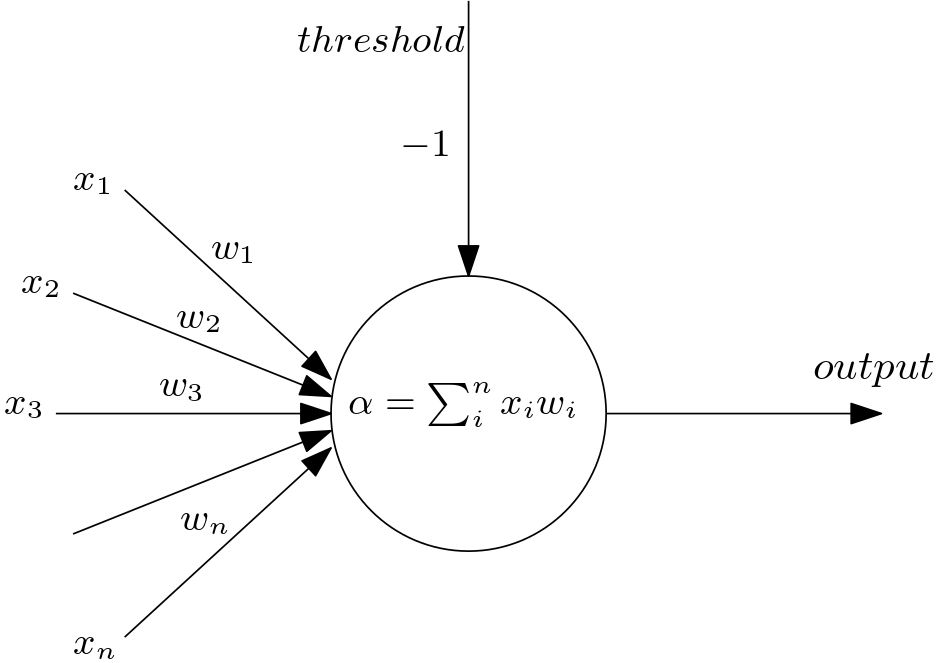
\includegraphics[width=12cm]{perceptron.png}
	\caption{Perceptron \cite{matous}}
	\label{fig:perceptron}
\end{figure}

%=======================================================================================================================
\subsection{Sigmoid Neuron}
Sigmoid neuron, similarly to perceptron, has inputs x and weights. The key difference comes in once we inspect the output value and its calculation.
 Instead of perceptron's binary output 0 or 1, a sigmoid neuron outputs a real number between 0 and 1 using a sigmoid function. \newline
[http://neuralnetworksanddeeplearning.com/chap1.html][8M] \newline
MATH\\
PLOTS\\

As shown in Figure xx and Figure xx, the sigmoid function is a smoothed-out version of the step function.\\
%=======================================================================================================================
\subsection{Activation Function}
An artificial neuron's activation function defines that neuron's output value for given inputs, commonly being ${f: \mathbb{R} \rightarrow \mathbb{R}}$ \cite{leskovec2020mining}. A significant trait of many activation functions is their differentiability, which allows them to be used for \textit{Backpropagation}, ANN algorithm for training weights. The activation function needs to have a derivative that does not saturate by heading towards 0 or explode by heading towards inf \cite{matous}.

For such reasons, the usage of step function or any linear function is unsuitable for ANN.
% Sigmoid Function ==========================================================================================================
\setsecnumdepth{all}
\subsubsection{Sigmoid Function}
The sigmoid function is commonly used in ANN as an alternative to the step function. A popular choice of the sigmoid function is a \textit{logistic sigmoid}. Its output value is in the range of 0 and 1.

\begin{equation}
    {\sigma(\alpha) = \frac{1}{1 + e^{-\alpha}} = \frac{e^x}{1 + e^{x}}}
\end{equation}


% \begin{figure}[h]
%   \centering
%     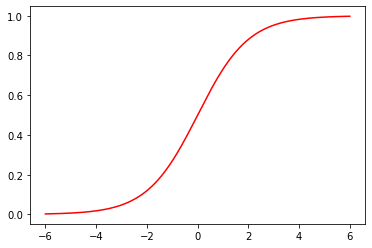
\includegraphics[width=7cm]{sigmoid}
%   \caption{Sigmoid function}
%   \label{fig:sigmoid}
% \end{figure}


One of the reasons for its popularity is the simplicity of its derivative calculation:

\begin{equation}
    {\frac{d}{dx}\sigma(\alpha) = \frac{e^x}{(1 + e^{x})^2} = \sigma(x)(1-\sigma(x))}
\end{equation}


On the other hand, one of its disadvantages is the \textit{vanishing gradient}. A problem where for a given very high or very low input values, there would be almost no change in its prediction. Possibly resulting in training complications or performance issues \cite{7typesactivationfunctions}, \cite{matous}.

% Hyperbolic Tangent ==========================================================================================================

\subsubsection{Hyperbolic Tangent}

Hyperbolic tangent is similar to logistic sigmoid function with a key difference in its output, ranging between -1 and 1.

\begin{equation}
    {tanh(x) = \frac{e^x - e^{-x}}{e^x + e^{-x}}}
\end{equation}


\begin{figure}[h]
    \centering
    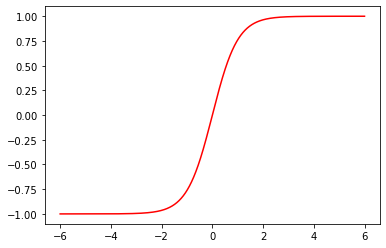
\includegraphics[width=8cm]{tangent}
    \caption{Hyperbolic tangent \cite{matous}}
    \label{fig:hyperbolictangent}
\end{figure}


It shares the sigmoid's simple calculation of its derivative.

\begin{equation}
    {\frac{d}{dx}\tanh(x) = 1 - \frac{(e^x - e^{-x})^2}{(e^x + e^{-x})^2} = 1 -\tanh^2(x)}
\end{equation}

By being only moved and scaled version of the sigmoid function, hyperbolic tangent shares not only sigmoid's advantages but also its disadvantages \cite{leskovec2020mining}, \cite{matous}.

% Rectified Linear Unit ==========================================================================================================

\subsubsection{Rectified Linear Unit}

The output of the Rectified Linear Unit (ReLU) is defined as:

\begin{equation}
    f(x) = max(0,x)
\begin{cases}
    x, & \text{if $x\ \geq\ 0$}\\
    0, & \text{if $x\ <\ 0$}
\end{cases} 
\end{equation} 

\begin{figure}[h]
    \centering
    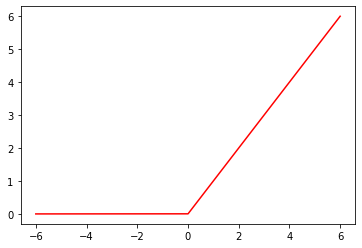
\includegraphics[width=7cm]{relu}
    \caption{Rectified Linear Unit \cite{matous}}
    \label{fig:relu}
\end{figure}


ReLU's popularity is mainly due to its computational efficiency \cite{7typesactivationfunctions}. Its disadvantages appear when inputs approach zero or to a negative number. Causing the so-called dying ReLu problem, where the network is unable to learn. There are many variations of ReLu to this date, e.g., Leaky ReLU, Parametric ReLU, ELU, ...
% Softmax ==========================================================================================================

\subsubsection{Softmax}

Softmax separates itself from all the previously mentioned functions by its ability to handle multiple input values in the form of a vector $\vec{x} = (x_1,x_2,...,x_n)$ and output for each $x_i$ defined as:

\begin{equation}
    {\sigma(x_i) = \frac{e^x_i}{\sum_{j=1}^{n}e^x_j}}
\end{equation}


For output being normalized distribution probability distribution, which ensures $\sum_{i}\sigma(x_i) = 1$ \cite{lipton2015critical}. It is being used as the last activation function of ANN to normalize the network's output into $n$ probability groups.

%=======================================================================================================================
%=======================================================================================================================
\section{Types of Neural Networks}
A
B
C
%=======================================================================================================================